\documentclass{article}
\usepackage{assignment_preamble}

\title{Lab 2}
\author{Ravi Kini}
\date{October 29, 2023}

\begin{document}

\maketitle

\repository{https://github.com/ravidosa/notes/tree/main/academics/assignments/code/phy112l_lab2}

\problem
The free energy $F$ and entropy $S$ are
\begin{equation}
    \begin{split}
        F & = -k_B T \ln Z \\
        S & = \frac{1}{T}\left(\langle E \rangle - F\right)
    \end{split}
\end{equation}
The free energy is also written as
\begin{equation}
    F = \langle E \rangle - TS
\end{equation}
In the high-temperature limit, the entropy $S$ of a system with $N$ states becomes:
\begin{equation}
    \begin{split}
        \lim_{T\to\infty} S & = \lim_{T\to\infty} \frac{\langle E \rangle - F}{T} \\
        & = \lim_{T\to\infty} \frac{\sum_{n=0}^{N-1}p_n E_n + T\ln\mathcal{Z}}{T} \\
        & = \lim_{T\to\infty} \frac{\sum_{n=0}^{N-1}p_n E_n}{T} + \lim_{T\to\infty} \ln\mathcal{Z} \\
        & = 0 + \ln N = \ln N \\
    \end{split}
\end{equation}
For $N = 2$, $\lim_{T\to\infty} S = \ln 2$.
In the low-temperature limit, the entropy $S$ of a system with $N$ states becomes:
\begin{equation}
    \begin{split}
        \lim_{T\to 0} S & = \lim_{T\to 0} \frac{\langle E \rangle - F}{T} \\
        & = \lim_{T\to 0} \frac{\sum_{n=0}^{N-1}p_n E_n + T\ln\mathcal{Z}}{T} \\
        & = \lim_{T\to 0} \frac{\sum_{n=0}^{N-1}p_n E_n}{T} + \lim_{T\to 0} \ln(\sum_{n=0}^{N-1}e^{-\beta E_n}) \\
        & = \lim_{T\to 0} \frac{E_0}{T} + \lim_{T\to 0} -\beta E_0 + \ln(1 + \sum_{n=0}^{N-1}e^{-\beta (E_n - E_0)}) \\
        & = \lim_{T\to 0} \frac{E_0}{T} + -\frac{E_0}{T} + \ln(1 + \sum_{n=0}^{N-1}e^{-\beta (E_n - E_0)}) \\
        & = \lim_{T\to 0} \ln\left(1 + \sum_{n=0}^{N-1}e^{-\beta (E_n - E_0)}\right) = \ln 1 = 0 \\
    \end{split}
\end{equation}
For $N = 2$, $\lim_{T\to 0} S = 0$.

\clearpage

\problem
At high temperatures, systems have an equal $\frac{1}{N}$ probability of being in any of the $N$ states. The entropy is $\ln N$, and as there are $N$ accessible states, the statement holds. At low temperatures, systems must be in the $E_0$ state. The entropy is $\ln 1 = 0$, and as there are $1$ accessible states, the statement holds.

\clearpage

\skipproblem

\problem
Figure \ref{fig:fig1} is a plot of $S$ vs. $T$ for $N = 3$ and $E_0 = -3.7, E_1 = -3.5, E_2 = 0.5$. As $T \to \infty$, $S \to \ln 3 \approx 1.09$ and as $T \to 0$, $S \to 0$. This makes sense in terms of the results for Exercise 1. The entropy also has a steep increase whenever $E_n - E_0$ has a steep increase; here $E_1 - E_0 = 0.2$ and $E_2 - E_0 = 4.2$, and $S$ increases significantly around $T = 0.2$ and $T = 4$.
\begin{figure}[!htb]
    \centering
    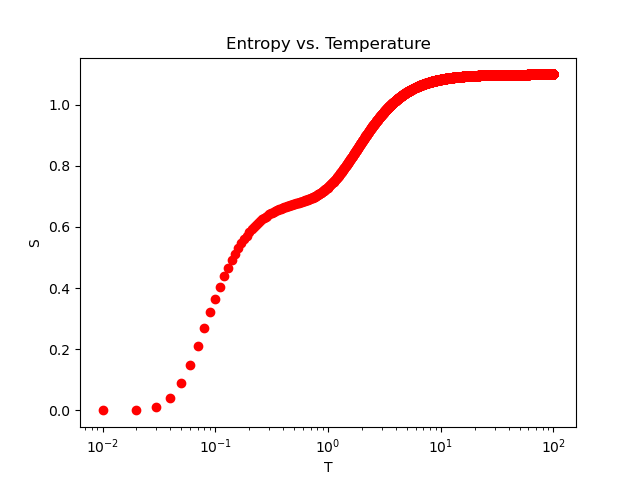
\includegraphics[width=0.75\textwidth]{../code/phy112l_lab2/2-4.png}
    \caption{Plot of entropy vs. temperature ($E_0 = -3.7, E_1 = -3.5, E_2 = 0.5$).}
    \label{fig:fig1}
\end{figure}

\clearpage

\problem
Figure \ref{fig:fig2} is a plot of $S$ vs. $T$ for $N = 7$ and $E_0 = 0.3, E_1 = 0.4, E_2 = 0.5, E_3 = 5.0, E_4 = 6.0, E_5 = 300.0, E_6 = 400.0$. As $T \to \infty$, $S \to \ln 7 \approx 1.95$ and as $T \to 0$, $S \to 0$. This makes sense in terms of the results for Exercise 1. The entropy also has a steep increase whenever $E_n - E_0$ has a steep increase; here $E_1 - E_0 = 0.1$, $E_3 - E_0 = 4.7$, and $E_5 - E_0 = 297.7$, and $S$ increases significantly around $T = 0.2$, $T = 5$, and $T = 300$.
\begin{figure}[!htb]
    \centering
    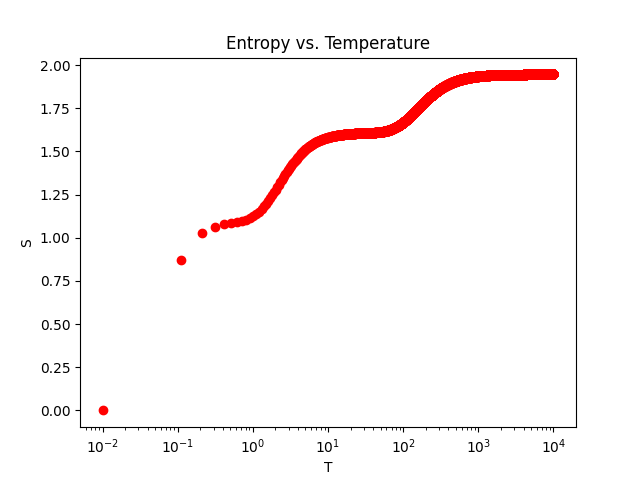
\includegraphics[width=0.75\textwidth]{../code/phy112l_lab2/2-5.png}
    \caption{Plot of entropy vs. temperature ($E_0 = 0.3, E_1 = 0.4, E_2 = 0.5, E_3 = 5.0, E_4 = 6.0, E_5 = 300.0, E_6 = 400.0$)}
    \label{fig:fig2}
\end{figure}

\clearpage

\problem
The entropy can also be calculated by integrating the specific heat.
\begin{equation}
    S(T) = \int_0^T \frac{C(T')}{T'} \, \diff{T'}
\end{equation}
Figure \ref{fig:fig3} is a plot of $S$ vs. $T$ for $N = 3$ and $E_0 = -3.7, E_1 = -3.5, E_2 = 0.5$. This makes sense in terms of the results for Exercise 1. The entropy also has a steep increase whenever $E_n - E_0$ has a steep increase; here $E_1 - E_0 = 0.2$ and $E_2 - E_0 = 4.2$, and $S$ increases significantly around $T = 0.2$ and $T = 4$. The entropies calculated using (1) and (5) agree, although the second method is very slightly off at high temperatures; this is likely because the size of the subintervals are too large for the trapezoidal method to be accurate.
\begin{figure}[!htb]
    \centering
    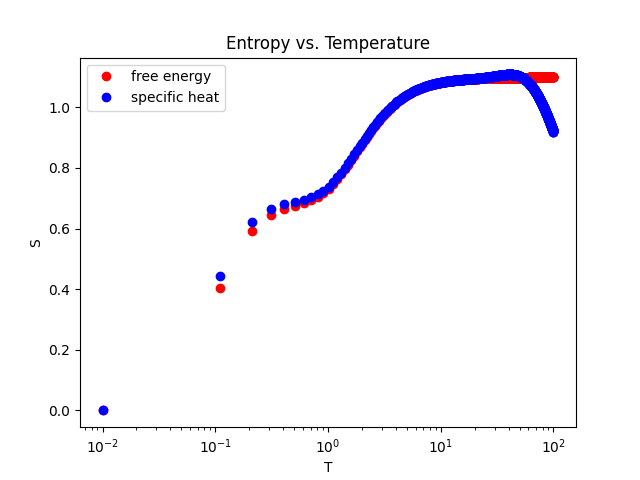
\includegraphics[width=0.75\textwidth]{../code/phy112l_lab2/2-6.png}
    \caption{Plot of entropy vs. temperature ($E_0 = -3.7, E_1 = -3.5, E_2 = 0.5$)}
    \label{fig:fig3}
\end{figure}

\end{document}